\documentclass[11pt,a4paper]{report}
\usepackage[english]{babel}
\usepackage[utf8]{inputenc}
\usepackage[T1]{fontenc}
\usepackage{glossaries}
\usepackage{graphicx}
\usepackage{hyperref}
\usepackage{wrapfig}
\usepackage{float}
\usepackage{natbib}
\usepackage{listings}
\usepackage{caption}
\usepackage{subcaption}
\newcommand{\HRule}{\rule{\linewidth}{0.5mm}}
\setlength\parindent{0pt} % Removes all indentation from paragraphs	 
%% Acronimos
%\newglossaryentry{sqlite}
%{
%  name=SQLite,
%  description={é um sistema de gestão de base de dados}
%}
%\newacronym{aes}{AES}{Advanced Encryption Standard}
%\newacronym{sha}{SHA}{Secure Hash Algorithm}
%\makeglossaries
%% Fim da introdução do Acronimos

\let\olditemize\itemize
\renewcommand{\itemize}{
  \olditemize
  \setlength{\itemsep}{1pt}
  \setlength{\parskip}{0pt}
  \setlength{\parsep}{0pt}
}

\title{\textbf{Identity Enabled Distribution Control System} \\1st Project\\ Segurança\\Universidade de Aveiro}
\author{Diogo Silva 60337 \and Tânia Alves 60340 }

\begin{document}
\begin{titlepage}
\begin{center}
\HRule \\[0.4cm]
{ \huge \bfseries Identity Enabled Distribution Control System \\[0.4cm] }
\HRule \\[1.5cm]
\textsc{\LARGE Universidade de Aveiro}\\[1.5cm]
\textsc{}\\[1.5cm]
\textsc{Diogo Silva 60337 \\Tânia Alves 60340 }
\end{center}
\end{titlepage}
\maketitle
\tableofcontents
\nocite{*}
\chapter*{Context}
\addcontentsline{toc}{chapter}{Context}
This project was done for Security, for the 2015/2016 lective year.
It aims to create an end to end secure digital rights management system to handle the distribution of video files, music files or books.

\chapter*{Introduction}
\addcontentsline{toc}{chapter}{Introduction}

Our project is made of two main components: the player and the server.
The server is in charge of controlling the user access to the protected files. 
The player requests and plays the files from the server.
In order for the user to have access to the titles he/she wants, we also have a web application where the user can buy the titles to play later.
To reach the goal of this project, we also needed a database that helped manage the user and file related information.

\begin{figure}[H]
\centerline{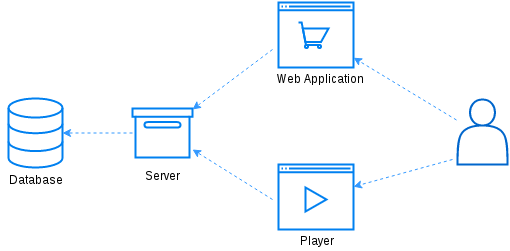
\includegraphics[width=300pt]{images/overview.png}}
\caption{Component overview}
\label{schema}
\end{figure}

%%%% CAPITULO RELATIVO A APLICAÇÃO %%%%
\chapter{System components}
This chapter includes information about the database we used to support the server.
We stored information about the users, files, players and devices that were later used.

\section{Database}
For the database we thought of this layout:

\begin{figure}[H]
\centerline{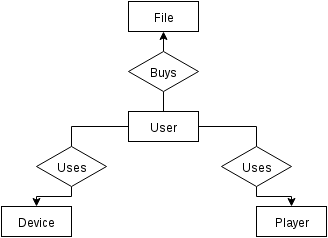
\includegraphics[width=200pt]{images/dbSchema.png}}
\caption{DB Schema}
\label{schema}
\end{figure}

We need to save information about the users that belong to the system and buy the files. 
The files that are stored in the server and are then sent to the players. The players that will interact with the server and play the files. And the devices where the users play the files.

\subsection{Database tables}
Using the information presented, we derived the tables for the database, with all the attributes necessary for our implementation of the system.

\begin{figure}[H]
\centerline{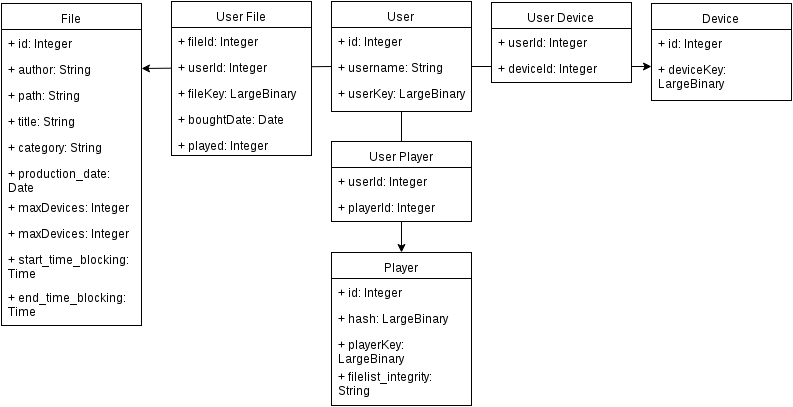
\includegraphics[width=500pt]{images/dbTables.png}}
\caption{DB Tables}
\label{tables}
\end{figure}

Each "main" entities (User, Device, File and Player) will have an id that identifies the entity in the database.
We then have the required key for each one of them as well.
\newline In the User table we have added the username field that identifies the each user. For the second part of the project, the username is literally the full name present in the authentication certificate extracted from the user's citizen card. Also, for this part of the project, we added an extra field that holds the hash of the user's authentication certificate.
\newline The File table also has some extra fields that provide information to the user about the file he is playing or buying, such as, the title of the file, the author, the category and the date of the title's production.
\newline The actions presented in Figure 1.1 had to be converted to extra tables since, in each case we had a many-to-many relationship. So, we have here the extra tables that store some information of the interactions, like specific keys and adittional information like the date that when the user bought the file. 
\newline Besides the tables presented before, we needed a few more tables to help implement the authorization policies:

\begin{figure}[H]
\centerline{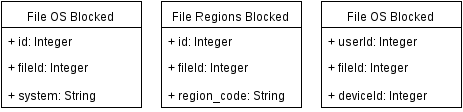
\includegraphics[width=300pt]{images/auxTables.png}}
\caption{DB Auxiliary Tables}
\label{tables}
\end{figure}

\subsection{Technologies used}
For the database we used:
\begin{description}
  \item[PostgreSQL] Open source, object relational database management system. We chose this over SQLite for example because it has a better support for storing secure data.
  \item[SQLAlchemy] Open source SQL toolkit. Works as an object-relation mapper for Python. This allowed us to create database scripts that created the tables and populated the database.
\end{description}

\section{Server}
The server is meant to interact with the database and control the access of the users and players to the files.
This interaction is done over a \emph{HTTP Rest} interface.
 
\subsection{Structure}
The server is composed of several files:

\begin{description}
  \item[Server file] This is the main file that holds the code to execute the server. When we want to start the server, it must be with \emph{sudo} because the server is using port 443 to host (which requires previligies).
  \item[Cipher file] This file holds auxiliary cryptographic functions that are used by the server.
  \item[Checker file] Holds auxiliary functions that make certain verifications before each request to the \emph{HTTP Rest API}, such as making sure the user is logged in before the player tries to download a file, or check if there's a device key reported when player logged in, etc.
\end{description}

\subsection{Implementation}
The server communicates with the player through \emph{SSL}. We did it like this so that we could focus on other parts of the system instead of implementing it from scratch.
For this, we needed to create certificates for both server and players.
\newline CherryPy does not run SSL communications natively so, we needed to use Apache to create a proxy for the CherryPy server. The requests are caught by the Apache server and sent to CherryPy to be proccess. The responses to these requests are then sent back to Apache and returned to the client.

\subsection{Technologies used}
\begin{description}
  \item[Apache] Free, open source web server that contains modules for TLS, SSL, proxy, ... Which is exactly what we need to have a fully functional HTTPS proxy.
  \item[CherryPy] Object oriented web application framework for Python. We chose this because it is built for rapid development of web applications and offers the basic configurations, that is what were looking for.
  \item[psycopg2 package] This is a Python-PostgreSQL database adapter that manages context, diagnosis errors and more.
  \item[OpenSSL] Toolkit that implements SSL and TLS protocols with cryptographic support. We used this so that we could create a certain level of abstraction on how the communications were made, and like that, we could focus in the rest of the system.
\end{description}

\section{Web page}
The web page is where the user can buy the titles.
It requires the user to log in with the citizen card before proceeding with the titles purchase.
The same API that the player uses is used here.

\begin{figure}[H]
\centerline{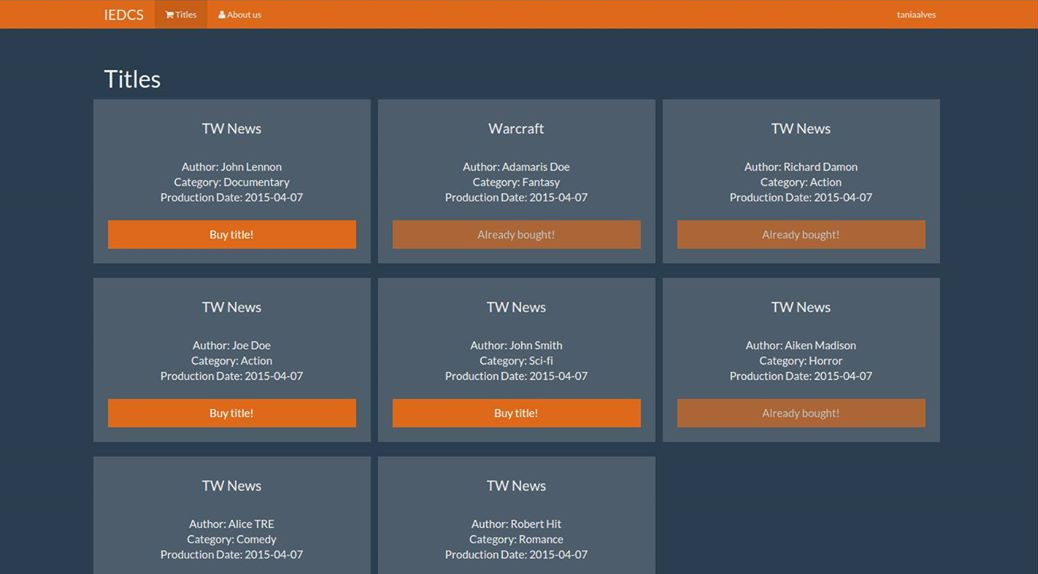
\includegraphics[width=500pt]{images/webpage.jpg}}
\caption{Web page interface}
\label{webpage}
\end{figure}

It is a simple interface that has a button to buy a specific title.

\section{Player}
The player allows the user to play the files he/she has bought previously through the WebPage. 
\newline  In this implementation we used video files in order to prove that our implementation can handle big files.

\subsection{Structure}
The player implementation we have is made of 5 main files. 

\begin{description}
  \item[Player file] This file contains the mainloop for the player's graphical interface. It is here where most of the requests to the server and main operations are made.
  \item[Playback file] The playback file contains the code that actually plays the file. The decryption is done here, block by block and fed to the thread that runs a VLC player instance.
  \item[My List file] This file is an auxiliary file that defines the structure of the list that the player displays to the user containing the titles the users owns. This is only to improve the appeareance of the list.
  \item[videos folder] This folder is where the player stores the encrypted videos. Inside, there is another folder for each user that uses the player named after his/her username. This method was chosen so that it is easy for each player to go and grab the files that belong to him/her if he/she chooses to move the files and use another player or device.
  \item[CC utils file] This auxiliary files contains methods that allow interact with the citizen card.
\end{description}

\subsection{Implementation}

The player garantees to the server that the its code was not altered by the user and the server knows how it is implemented. For that the integrity of the player is validated. This validation consists in a exchange of messages between server and player, in \autoref{sec:integrity} the details of this validation are presented with more detail.
After the user starts the player application, he/she must log in. 

\begin{figure}[H]
\centerline{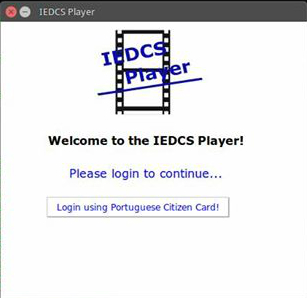
\includegraphics[width=200pt]{images/playerLogin.jpg}}
\caption{Login page for the player}
\label{player}
\end{figure}

For the user to login, the citizen card must be inserted in the card slot and the user must insert the pin code that corresponds to the authentication action. At this point, besides the user authentication certificate, we also send the Device Key (\autoref{sec:diagfile}) to the server alongside the Player certificate (\autoref{sec:certs}).
\newline After the user logs in and it is confirmed by the server, a list of titles is displayed so that the user can choose which one he/she wants to reproduce.

\begin{figure}[H]
\centerline{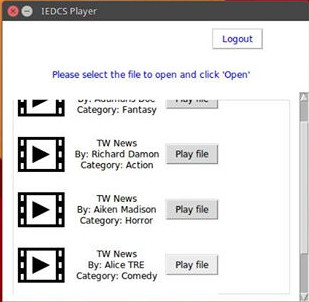
\includegraphics[width=200pt]{images/playerList.jpg}}
\caption{Page that lists the files for the user}
\label{player}
\end{figure}

When the user selects the file that he/she wants to play, a thread running the VLC player is started. The thread reads blocks of the encrypted file, decrypts it and sends it to the VLC buffer.
The player gets the file through a stream instead of a simple \emph{GET} request, so that large files can be played immediately.
At this point, several other validations are performed: policies, player certificate validation, player integrity (from before), and Device Key (also from before - This service is referenced in more detail at \autoref{sec:requ}).
\newline
The buffer is managed by the VLC player and is customizable (the user can give the buffer the size it wants by changing the value on the VLC settings).

\begin{figure}[H]
\centerline{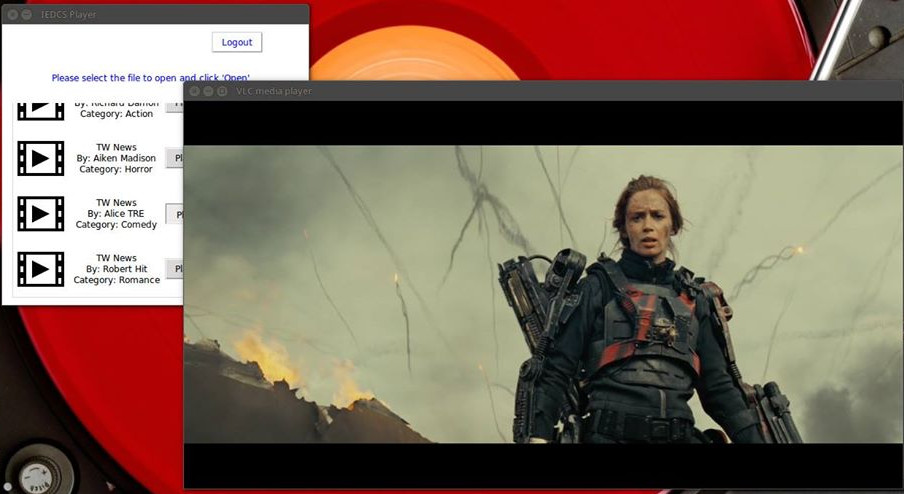
\includegraphics[width=300pt]{images/playerPlay.jpg}}
\caption{Video playing in the VLC thread}
\label{player}
\end{figure}


All the requests done to the server are performed over the server's \emph{HTTP Rest} API that was presented earlier.

\subsection{Technologies used}
\begin{description}
  \item[Tkinter] We built the graphical interface with Tkinter that is the Python graphic user interface framework.
  \item[VLC Player] To make things a bit easier when handling video files, we used the VLC player that takes care of the video format encoding.
  \item[Python requests package] This package enabled us to communicate with the server producing requests and receiving responses.
  \item[PyCrypto package] This is the package that helps handle encryptions and decryptions.
  \item[M2Crypto package] This package was used to get information from the citizen card.
\end{description}

\chapter{System keys}
\section{Player Key}
This is a key that must be generated after each code is evaluated by the company that wants to implement the system. 
This evaluation checks if the player, and the respective code, meet the security requirements. 
Taking into consideration when it is generated and the process behind it, this key ensures that the player works accordingly to the security policies.
\newline At this stage, the player was generated from a random array of bytes and stored in the database, on the server side, since we are the ones that are devoloping the player.
In the player, the Player Key is hardcoded.
\newline This key is present in the server and in the player.
Besides that, a certificate for the player is generated so that we can guarantee its authenticity and we can also associate the player that the user is using to the Player Key. As such, there is no way to reproduce files without the player having a valid certificate.

\section{Device Key}
The Device Key is a key that identifies the device where the player is being executed. This key should be the same even if the we have more than one player running in a device.
In the Device Key generation, there were some dificulties in finding the best solution.
\newline We wanted to use the processor serial number because we know that the number we get is already unique.
However, this is an information that is hard to get. We came across the command \emph{cpuid} that is used in linux systems, but the Python wrapper available, \emph{Pycpuid}, requires an option to be enabled on BIOS to check the CPU UUID (not everyone has it enabled).
We also thought about the MAC Address but it was automatically discarded since MAC Address can be modified easily.
\newline We then turned to the command \emph{dmidecode} that gives us a list of device informations that could be used. 
Yet again, we found an obstacle. To access the processor serial number, we needed to run the player with \emph{sudo} which goes against one of the principles of security ("No entity should have greater permissions in the system other than basic permissions it needs to perform its tasks").
So, with some research we found that the information the \emph{dmidecode} command provides is stored in some system files, specifically, in the \emph{/sys/devices/virtual/dmi/id/} directory.
We then browsed all the files present in the directory and came across the one file that didn't require \emph{sudo} to read. 
This file was the \emph{modalias}, that contained all the information gathered by \emph{dmidecode} that didn't require superuser permissions.
\newline So, for the device key generation, we read the file and hashed the entire content with SHA256, using its digest.
\newline In our solution, this key is generated when the user logs in the player and is sent to the server at this stage. So, the Device Key is present both in the player and in the server.

\section{User Key}
The User Key is a key that identifies the user in the server. 
In our implementation, this key is generated when the user registers in the web page and is then stored in the database along with the rest of the user information gathered.
This key is only ever present in the server, and, as we will see, this will be part of the step that forces the player to communicate with the server each time a file is played.

\section{File Key}
This key identifies the file that the user bought and is independent of the device and player. When compared to the rest of the keys, this one requires a bit more work to derive.

\begin{figure}[H]
\centerline{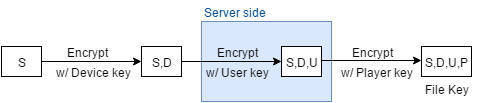
\includegraphics[width=300pt]{images/fileKey.png}}
\caption{Derivation process for the File Key}
\label{fileKey}
\end{figure}

As we can see from the previous diagram, the File Key is derived from the previous keys presented by encrypting them in a chain of operations.
We used the AES algorithm for this.
\newline In the server side, if it is the first file encryption that the server performs for that file and user, we have the following steps:
\begin{enumerate}
  \item The server generates a random start seed and a random initilization vector since we are going to use CBC to decrypt the file.
  \item It then performs the encryption chain presented above to get the resulting File Key.
  \item The server then encrypts the file with the result.
  \item The encrypted file and the start seed are sent to the player so that it can decrypt the file.
  \item The server stores the File Key and the initilization vector (IV) in the database.
\end{enumerate}

If the file has already been sent at least one time, the steps change a bit:
\begin{enumerate}
  \item The server gets the File Key stored in the database.
  \item It then performs the chain of encryption in reverse, decrypting the File Key with the rest of the keys that it has access at that time.
  \item The result will be the seed that was used to derive that File Key, and so, it is sent to the player.
\end{enumerate}

This chain allows the player to derive the File Key, even if the device or/and player changes, because the information that the server sends to the player is the starting seed.
\newline In the player side, whatever the File Key is, the operation's chain is the same. However, the blue square present in the diagram above represents a step in which the player must include the server because it does not have access to the User Key.
\begin{enumerate}
  \item The player gets the seed (and IV used to decrypt file later) from the server and encrypts it with the Device Key.
  \item It then sends the result to the server and the server will encrypt it with the User Key, which the player does not have access to (to do this user must be correctly identified, in this case there must be a login associated to the session)
  \item The server sends the result back and the player will then encrypt it with the Player Key, resulting in the File Key.
\end{enumerate}

\chapter{Server-Client interactions (REST API detailed)}

\section{Summary}
All pre-validations of the services are in the \emph{checker.py} file that implements a wrapper that tells CherryPy what are the necessary verifications that it has to perform before each service (eg. @require(logged(), device\_key(), is\_player(), player\_integrity()) for the download. You can find this annotation in the top of the \emph{GET} request for the download operation).

\subsection{Player - Server}
The server-player interaction takes advantage of 7 different types of requests to the server:
\begin{enumerate}
\item GET /api/user/loginchallenge allows the player to get a challenge to initiate a session in the server, logging in the user. The server generates a random byte array and returns it to the user to be signed, confirming the user's identity. It requires the portuguese citizen to be able to use this function.
\item POST  /api/user/loginchallenge is sent with the following payload in json format: portuguese citizen auhentication certificate in PEM format, the challenge signed with the user's private key, authentication certificate common name and certificate root common name. 
    After the certificate is validated, this information will be associated with the current user session\_id, allowing us to keep a record of the login during the whole interaction/session. Besides these parameters, the player also sends the Device Key that it calculated.\\
    If the user fails to validate the challenge, it will need to request a new challenge.
\item POST  /api/user/logout that removes any association in the server to the session\_id (this operation requires a previous login, that is, the username must be associated with a session\_id before hand).
\item GET   /api/title/user/ that lists all the titles that the user purchased earlier (this operation also and only requires that the user is logged).
\item GET   /api/valplayer/ that returns a SALT which allows the server to perform the player's integrity validation.
\item POST  /api/valplayer/<hash> using the previous returned SALT, the player must send the locally calculated HASH and then the server will confirm if the result is the expected result or not (sort of a challenge).
\item GET   /api/title/<pk> receives a stream of the file's content (where <pk> is the title identifier of the file that the user wants to download). This is a critical operation in terms of system security because it can't be used if one of the following conditions fails: Existance of player's certificate, previously performed player integrity, the user is logged in, the player has already sent the Device Key.
\item POST  /api/title/validate/<hash> which it is used by the player to send to the server the HASH that it has at that moment. The server will then encrypt the HASH with the User Key and sends the result back to the player (this operation requires the same conditions presented in the previous item).
\end{enumerate}

\subsection{Webpage - Server}
The server-web page interaction is based in 5 different requests to the server:
\begin{enumerate}
\item POST  /api/user/login where the param is the device key. On the server side, the server will try to obtain the certificate used for the SSL communications that should be the citizen card certificate.
\item POST  /api/user/logout that removes any association in the server to the session\_id (this operation requires a previous login, that is, the username must be associated with a session\_id before hand).
\item GET   /api/title/all that lists all the titles available for purchase (does not require login).
\item GET   /api/title/user/all that lists all the titles available to the user, with more detail so that the user can purchase or just view them (this requires login).
\item POST  /api/title/<pk> where <pk> is the id of the title that will be purchased by the user (this operation also requires previous login).
\end{enumerate}

\section{Checking player integrity}
\label{sec:integrity}
Every time a player executes, an operation to check its integrity is performed. This falls into the authorization headers, however, we deal with it right off the start.\\

We get the files that belong to the player implementation and create a hash of each of the files. We then concatenate the hashes of each file and once more hash the result with a random generated salt and we get the final result.\\

The server generates a SALT and stores it to the session temporarily (SALT is discarded when the routine to validate is called or when requested to generate a new SALT), and sending it to the player. Player will execute the sequence of operations described before to generate the hash. The result will be compared with the information stored in the server, and if they are equal, the player's integrity will be confirmed, otherwise, we assume someone has altered the code and the player is rejected.

Two services are invoked:  
\begin{enumerate}
\item GET   /api/valplayer/ that returns a SALT that allows the server to validate the integrity of the player.
\item POST  /api/valplayer/<hash> that submits the result of the challenge (if it fails, the SALT is discarded and a new one must be generated).
\end{enumerate}

\section{Logging in}
To be able to perform any action, the user must first login. This is mandatory in both web page and player.
\newline For this, the server offers a login operation through the \emph{Rest API}

\begin{figure}[H]
\centerline{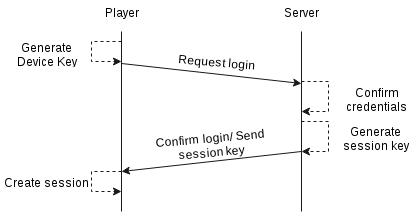
\includegraphics[width=200pt]{images/loginDiagram.png}}
\caption{Login interaction (player - server)}
\label{player}
\end{figure}

As we can see from the diagram above:
\begin{enumerate}
  \item The player starts by generating the Device Key for the device. \label{sec:diagfile}
  \item The player requests a challenge to the server.
  \item The player sends the response to the server containing generated Device Key, the user authentication certificate, the certificates common name, the certificate's root common name and the data received earlier from the server signed with the user's private key. 
  \item The server checks the certificate that the user sent and accesses the database to verify the information it received associating the Device Key to the user.
  \item The server sends the response that signals the operation was completed successfully.
\end{enumerate}

The communication between player and server is done using sessions. Before the player starts communicating with the server, a session is created with the \emph{requests} package for Python.
From now on, all communications will be performed over this session.

\section{Purchasing the file on the web page}
This operation requires the user to be logged in already and is only available in the web page.

\begin{figure}[H]
\centerline{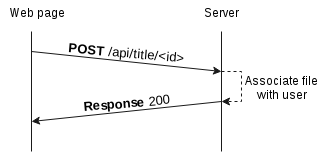
\includegraphics[width=200pt]{images/buyTitle.png}}
\caption{Purchase interaction (player - server)}
\label{player}
\end{figure}

As we can see, the operation isn't complex and the only thing done here is the association of the purchased file with the user.
This association translates in a new entry in the UserFile table in the database.

\section{Downloading the file from the player}
In this interaction, we have two distinct situations:
\begin{enumerate}
  \item Full file download
  \item Cryptographic information download
\end{enumerate}

\subsection{Download requisites (validations)}
\label{sec:requ}
So that the download of a file is possible, a few criteria must be met:
\begin{enumerate}
\item The user must be logged in.
\item The Device Key must be reported to the server on the login operation.
\item The player's authenticity must be validated (with the help of the certificate \autoref{sec:certs}, which will allow the server to associate the Player Key to session).
\item The player's integrity must be validated.
\item The user must have purchased the file previously through the web page.
\item The file for the user must meet all the policies imposed.
\end{enumerate}
The criteria verification has the order presented.

\subsection{Full file download}
The full file download situation means that this is the first time the player downs the file the user selected.
And so, the server must send back the full encrypted file along with the cryptographic information that will allow the player to decrypt the file.

To decrypt/encrypt the key, we used CBC, so, an IV is part of the cryptographic headers as well, even though we used streams to download the file (enabling large files to reproduce as well without the processing time of the encryptino being noticeable).
We chose CBC because CHerryPy's stream is done over TCP, that means that all data is guaranteed to treach the player. If it was done over UDP, we would probably choose CTR because there is no dependency between blocks in the encryption operation and we have random access to the file. 

\begin{figure}[H]
\centerline{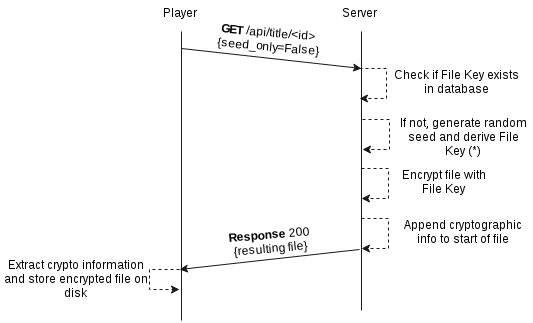
\includegraphics[width=200pt]{images/fullFileDown.png}}
\caption{Full file download (player - server)}
\label{player}
\end{figure}

(*) In this operation, there can be yet another two situations:

\begin{enumerate}
  \item The server has no File Key stored in the database, which forces the server to generate a random start seed to derive the File Key from. It then sends the seed with the encrypted file.
  \item The server already has a File Key stored, and it must derive the starting cryptographic information to send to the player, along with the file.
\end{enumerate}

\subsection{Cryptographic information download}
This situation only occurs if the player has already downloaded the file and has it stored on the disk.

\begin{figure}[H]
\centerline{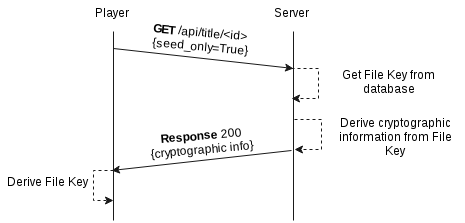
\includegraphics[width=200pt]{images/seedOnlyDown.png}}
\caption{Seed only download (player - server)}
\label{player}
\end{figure}

\section{Logging out from the player}
Logging out is a simple operation that only implies ending the session in the server.

\begin{figure}[H]
\centerline{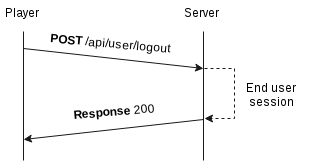
\includegraphics[width=200pt]{images/logout.png}}
\caption{Logout interaction (Player/Webpage - Server)}
\label{player}
\end{figure}

\chapter{TLS Socket and Certificates}
\label{sec:certs}
To guarantee that the communications channel is secure, we decided to the use a TLS Socket because it takes care of the channel encryption in a secure manner. This involves some criteria as well, such as the adequate generation of certificates.\\

All certificates were generated using XCA.
We have generated a Root Certificate Authority (CA) that is the issuer of all the certificates presented in this report and contains the following fields:
\begin{enumerate}
\item CN - Security P3G1 Root
\item ST - Aveiro
\item L - Aveiro
\item O - Universidade de Aveiro
\item OU - Departamento de Electrónica, Telecomunicações e Informática
\end{enumerate}
We also thought of the URI to a CRL that isn't being used at the moment, however, can be used later on to revoke certificates.

\section{CherryPy Server SSL Certificate}

For the CherryPy, a certificate issued by the Root CA had to be generated so that the chain of certificates can be guaranteed to work for any player, logged in user or browser. The CherryPy SSL adapter also had to be altered so that it supported client certificates (if present), for reasons that will be explained later.

\section{Players SSL Certificates}

We chose to generate certificates for each player so that the player validation could be performed and associated with a Player Key. This is the reason why we needed to change the builtin SSL adapter from CherryPy, supporting like this peer validation, since the default doesn't verify anything on the client side.

Being that the certificate is an optional step, if the client chooses not to use them, it cannot download files, nor request the chain of operations to derive the File Key.

\section{Browser validation}
For the browser we specified which CA of our DRM so that the browser can recognize the CA as trusted and trust all its issued certificates.

\chapter{Policies}
The policy validation is performed when the player tries to download the file (only after ensuring that its all good with the player, this is presented with detail at  \autoref{sec:requ}).
\begin{enumerate}
\item Limit the number of devices where the file can be reproduced. This information is stored in an auxiliary table in the database that associates the file with the devices allowing us to keep a track of the number.
\item File only valid for a certain region (the region detection is done based on Remote-Addr available in the HTTP request headers).
\item File only valid for a certain OS (the detection is done based in the User-Agent available in the HTTP headers, filtering the OS information).
\item Limit the time of the day the file can be reproduced (the time calculation is done server side).
\item Limit the number of times the file can be reproduced (there is a counter on the number of file plays).
\end{enumerate}

\chapter{Secure file storage}
To have a secure file storage for the server media files, we decided to take the approach of the file system level security presented in the practical classes. Even though the attacker will have access to the metadata of the files and the file system structure, this information is mostly available on the WebPage for any person to browse, so, there is no need to use this step.
\newline
To achieve this secure storage feature, we used the \emph{encfs} command that creates a mount point to where the files are sent and are then encrypted.
\newline
It was our goal to automate this whole process and so, we created a script using \emph{expect} (tool to automate interactive applications such as telnet, ftp,...) that allowed us to simulate the interaction needed to configure \emph{encfs}, that script is inside src/server/database/encfs.exp, it is used to create an encfs for a specific file.
\newline
We defined the structure of our file system taking into account that each user should have access what he/she needs, and nothing more.
\newline
For this, we divided the files in different folders and create a mount point for each file that we are accessing. Only the needed file is decrypted when the access to it is required, it will mount the specific file using \emph{encfs} and after 1 minute of inactivity it will unmount by itself, allowing multiple users requesting and using the same file at the same time.
\newline
The tool \emph{encfs} requires a password to be defined when the configurations are performed. Since each file is encrypted in a separate directory, we decided to gather the information present in the database concerning the file and add a random array that is hardcoded in the server.

\chapter{Confinement}

Supondo que queremos proteger o nosso servidor/estrutura onde o nosso serviço está instalado caso seja invadido, existe a necessidade de criar um confinamento para os nossos serviços, neste caso existe 3 serviços bastante importantes:
\begin{enumerate}
\item Apache (que é responsável por autenticar com o cartão de cidadão e servir de proxy para o CherryPy)
\item CherryPy (servidor web)
\item PostgreSQL (base de dados)
\end{enumerate}

Para o confinamento optou-se por um container Docker, sendo que foi desenvolvido um Dockerfile que permite instalar todo o sistema (não inclui o player, não fazia sentido incluir o player num servidor).\\
Convém referir também que o Docker quando é criado pela primeira vez cria a base de dados com os ficheiros na pasta server/media, no entanto também os elimina logo após estarem no disco encriptado.\\
Para além do Dockerfile, ainda é disponibilizado um script ``iecds-server\_run.sh'' que permite executar 4 comandos distintos sobre a instancia do docker:
\begin{enumerate}
\item start - Este comando inicia a instância do Docker caso ainda não esteja a correr
\item stop - Pára a instância do Docker caso esteja a correr
\item status - Permite verificar o estado actual do Docker
\item reset - Permite criar a instância novamente, sendo que a base de dados é eliminada e criada novamente aqui
\end{enumerate}

\chapter{System vulnerabilities review}
\section{SQL Injection}
QL Injection is a technique where malicious users can inject SQL commands into a SQL statement via inputs.
\newline
Using the developed player, the user can only enter his/her username and pin. Every other operation is performed with clicks, confining the user to the defined choices.
\newline
However, having the operations based on a HTTP Rest API, the user can still try to interact with the interface through command line or similar. We will then revisit the details of the REST API used:

\begin{enumerate}
 \item /api/title/login: This operation is a POST to the server that includes parameters such as username however, no information is inserted into the database.
 \item /api/title/logout: Even though this operation is also a POST, there is no information attached to it. It serves only the purpose of telling the server to close the user session.
 \item /api/title/user: This is a GET that returns all the titles bought by the user. There are no parameters since the user already has a session at this stage. This represents no harm.
 \item /api/valplayer/<hash>: Here, there is a POST request that takes a parameter that is the player hash that once again inserts no information in the database. Also we have a similar GET request (/api/valplayer) that takes no parameters.
 \item /api/title/<id>: This a GET request that takes the title id as a parameter. A verification is made here to ensure that the parameter received is indeed an integer. If it is something else other than an integer, the server automatically returns an error code as we can see in figure XX. We have a similar request to this one that is a POST used by the webpage, enabling the user to buy the specified title.
 \item /api/title/validate/<hash>: This POST request takes in a single parameter that is the hash the player derived so far. The only thing done here to the parameter is an encryption and it is then sent back to the player. There is no database interaction directly with the database.
 \item /api/title/user/all: This GET request takes no parameters as it only lists all the titles available to purchase.
\end{enumerate}

There is not much room for injection in our API, however, in our case, we used the SQLAlchemy toolkit for the database interactions, as mentioned before. This toolkit automatically escapes the characters used in database queries, ONLY IF the queries aren’t performed in raw form. To take advantage of this functionality we used only built in operations to INSERT, MODIFY or DELETE information from the database, never using raw built queries.
\newline
However, having the operations based on a HTTP Rest API, the user can still try to interact with the interface through command line or similar. We will then revisit the details of the REST API used:
We have some examples of tests we performed to try and explore the vulnerabilities. (This was a simple python script that was changed with different values and ran)

\begin{figure}[H]
\centerline{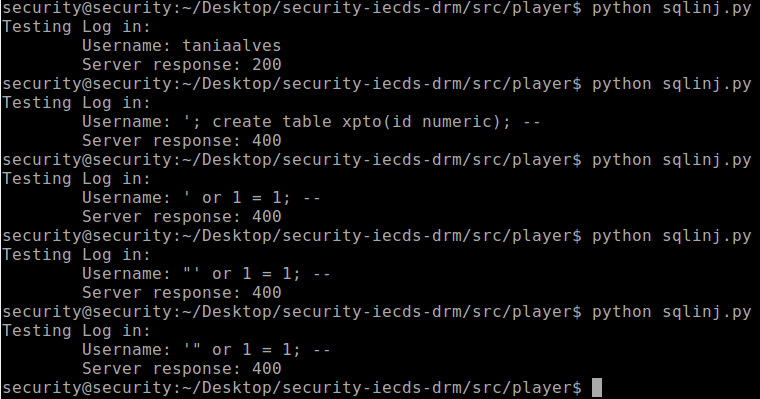
\includegraphics[width=200pt]{images/loginTest.png}}
\caption{This was a login attempt. The first result was a successful login, with an existing user, which results in a 200 response code (status OK). In the next attempt, we try to create a table by sending a CREATE SQL command. This produces a 400 status response (BAD REQUEST status), which means that the server did not find the user we tried. In the three next attempts, we try to force the login, however, the response is the same BAD REQUEST status.}
\label{player}
\end{figure}

\begin{figure}[H]
\centerline{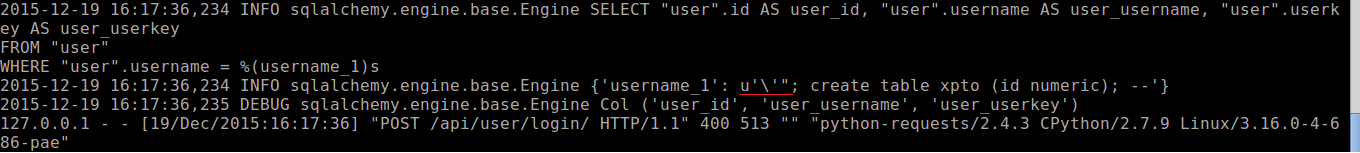
\includegraphics[width=200pt]{images/escapedChar.png}}
\caption{In this figure we have the server information displayed when it tries to search for the user ‘; create table xpto (id numeric); -- . We can see here that the character that finishes the string to start the command is escaped with a \ by SQLAlchemy (underlined with a small red line), and so the whole command is treated as a simple string.}
\label{player}
\end{figure}

\begin{figure}[H]
\centerline{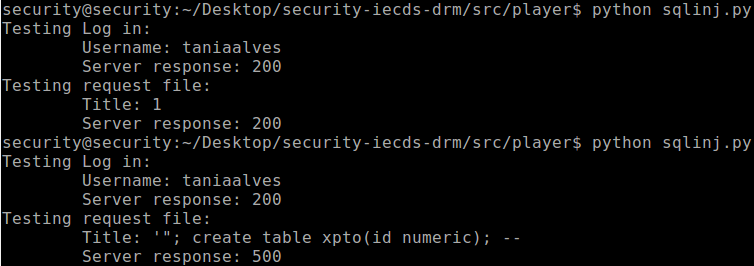
\includegraphics[width=200pt]{images/requestTitleTest.png}}
\caption{In this example, we tried to inject code through the title request, considering that we are already logged in. So, for the login, we had a successful request, however, if the title is not a integer, we receive a 500 (INTERNAL ERROR) status code in the response, as it is trying to convert the string to an integer.}
\label{player}
\end{figure}

\section{Buffer Overflow}

Attackers can use buffer overflows to corrupt the execution stack of an application by sending custom input to the application, enabling him/her to execute code that can for example open a command shell and allow him/her to take over the machine.
This attack relies on write access to particular memory addresses and the system mishandling data types.
Essentially every platform is vulnerable to this attack with the exception of:

\begin{itemize}
 \item Java / J2EE – As long as system calls or native methods are avoided
 \item .NET – as long as the developer stays away from unsafe or unmanaged code such as using P/Invoke or COM Interop
 \item PHP, Python, Perl – As long as the developer does not rely on vulnerable extensions or other vulnerable programs.
\end{itemize}

For this project we used Python alone throughout the functionalities. Python does not allow direct memory access and it is a strongly typed language (the definition for this is a fray area, however, we can that it is because the interpreter keeps track of all the variable types and so, it is the programmer’s responsibility to use the variables correctly).

Even though Python is “immune” to such attacks, it settles on a C language base, having its source code written in C, which is a vulnerable language because of allowing direct memory access and not being a strongly typed language. This is a concern because we have found some problems that, having its origin in the C code, propagate to the Python language as well.

We will go through a few problems found along the way in several versions of Python: (https://lwn.net/Alerts/651990/)

\begin{itemize}
    \item CVE–2014-1912: the function \emph{socket.recvform\_into()}, from the Modules/socketmodule.c module, failed to check the size of the supplied buffer for the receiving socket. This led to a security flaw and was present in Python 2.5 through 2.7.7, Python 3.x before 3.3.4 and Python 3.4.x before 3.4rc1. For this project we used the Python 2.7.9 version, so, being introduced after 2.7.7, the problem was fixed by adding a simple size check of the received information. (https://yazadk.wordpress.com/2014/12/10/remotely-exploitable-buffer-overflow-in-python/)
 \item CVE-2013-1752: multiple standard library modules implementing network protocols such as httplib and smtplib failed to restrict the sizes of server responses. This CVE actually is made of several issues for httplib, and even though we use requests, these are based on httplib. We also found that all the issues belonging to this CVE were fixed for version 2.7 and 3.1.
 \item There are other issues that will not be addressed here that were already corrected in Python versions prior to 2.7.9.
\end{itemize}

Some of these issues, even if not solved in the versions of Python could be solved by recompiling Python’s source code with canaries in the C compiler.

\section{Cross scripting}

\chapter{Installation}

There is an install script available in the root folder of the repository that was done in Ubuntu 15.04 and tested in the 14.04 e 14.10 versions (the password for the PostgreSQL can be found in the same file, commented out).\\

During the instalation, the user interaction will be requestes several times, for operations like selecting a certificate to install on the system, or the input for the database password.\\

A clone of a VM image was generated, however it has a size of 3.7GB (non zipped), with this being said, we chose not the upload it to the repository. Either way, it can be available to the teacher if problems are encountered.

\chapter{Conclusions}

There were some problems through out the project, like the Device Key generation, or the player validation using certificates because CherryPy doesn't support client certificate validation on its builtin adaptor (which originatesd the override of the class).\\

However these problems were solved after some work and the final goal was reached. 

%\printglossaries
%\addcontentsline{toc}{chapter}{Glossário}

\bibliographystyle{plain}
\bibliography{proj2}
%\addcontentsline{toc}{chapter}{Bibliografia}

%\listoffigures
%\addcontentsline{toc}{chapter}{Lista de figuras}
%\listoftables
%\addcontentsline{toc}{chapter}{Lista de tabelas}

\end{document}
